\documentclass[Rapport/Rapport_main.tex]{subfiles}
\begin{document}
\section{Krav}
\subsection{Introduktion}
I dette kapitel præsenteres de krav der er til Beer Pong-bordet. Der laves en beskrivelse af de regler for spillet, som der er defineret for lige netop dette Beer Pong-bord. Derudover laves en beskrivelse af funktionelle krav for bordet, hvori de forskellige brugstilfælde(Use Cases) forklares. Til sidst laves en beskrivelse af de ikke-funktionelle krav der er til bordet, altså de krav der beskriver bordets karakteristik fremfor bordets anvendelse. Til at starte med er det vigtigt at få defineret reglerne for spillet så de er afklarede. Her bruges mange definitioner fra Definitionslisten, så det er vigtigt at referere hertil.
\subsection{Regler for Beer Pong bordet}
Til at starte med skal bordet være klar til brug, hvilket er opfyldt ved, at bordet har kørt system rutinen \textit{start op}. Hvis bordet er klar til brug, så skal hvert \textit{hold} placere 6 kopper på hver side af bordet. Et \textit{hold} består af 2 brugere, og der er 2 \textit{hold} på hver deres side af bordet. Efter placeringen af kopper er \textit{spil præperationen} udført, og det er op til holdene at bestemme hvem, der starter med \textit{turen}. Desuden har holdene indtastet \textit{spiller oplysninger} ind. \\\\
\textit{Spillet er i gang} nu, hvorefter hver spiller på det \textit{aktive hold} kaster en bold af gangen. Hvis kun en bold rammer i en af \textit{modstander holdets} kopper, så skal \textit{modstander holdet} drikke indholdet af denne kop. Hvis begge bolde rammer i 2 forskellige kopper, så drikkes indholdet af begge kopper. Hvis begge bolde rammer i samme kop, så drikkes denne kop, samt to vilkårlige kopper. Efter det \textit{aktive hold} har kastet deres bolde, er de ikke længere i besiddelse af boldene, og rollerne som aktivt- og modstander-hold bytter.\\\\
Dette fortsætter indtil \textit{spillet er slut}, hvilket vil sige en af holdenes sidste kop er ramt. \textit{Det vindende hold} er så det hold, der rammer den sidste kop, og det holds resterende kopper drikkes af\textit{ modstander holdet}, der så er det \textit{tabende hold}. Reglerne er også blevet visuelt defineret i et flow chart diagram, der kan ses på figur \ref{fig:rap_beer_pong_flow}.
\begin{figure}[H]
    \centering
    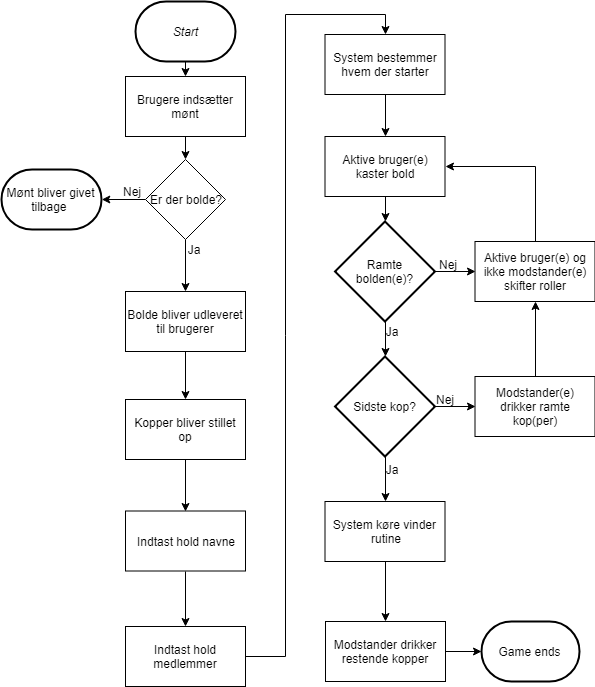
\includegraphics[width=0.8\textwidth]{Kravspecifikation/Flowchart/pics/Beerpongflowchart.png}
    \caption{Flow Chart diagram for et spil Beer Pong}
    \label{fig:rap_beer_pong_flow}
\end{figure}
Nu hvor reglerne er definerede, kan man begynde at gå i dybden med, hvordan Beer Pong bordet skal anvendes, hvilket er beskrevet gennem de funktionelle krav for bordet.

\subsection{Funktionelle krav}
I dette afsnit beskrives det funktionelle aspekt af bordet, hvem aktørerne til bordet er og hvordan det anvendes.
\subsubsection{Aktører}
Til at starte med er det værd at definere, hvem og hvad der kommer til at anvende bordet og hermed også påvirke det. Derfor er der som det første et Aktør-kontekst diagram, der beskriver dette, som kan ses på figur \ref{fig:rap_actor_context}.
\begin{figure}[H]
    \centering
    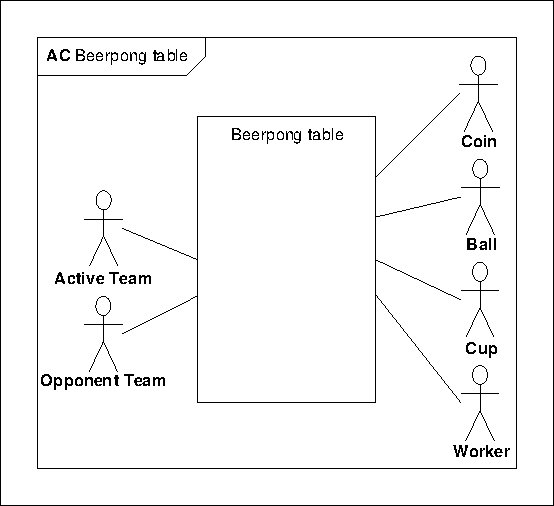
\includegraphics[width=0.7\textwidth,trim={0.24in 0.24in 0.24in 0.24in},clip, page=1]{Kravspecifikation/Funktionelle_krav/graphics_funktionel/Krav-spec-diagrammer.pdf}
    \caption{Aktør kontekst diagram for systemet}
    \label{fig:rap_actor_context}
\end{figure}
Af figur \ref{fig:rap_actor_context} ses de primære aktører til venstre, der skal symbolisere de to \textit{hold} der \textit{spiller} på bordet. Til højre ses de sekundære aktører, der er de andre udefra kommende ting der interagere med systemet. En \textit{mønt} starter spillet, en \textit{kop} registreres fjernet eller sat og en \textit{bold} registreres om den rammer i. Til sidst er der en \textit{arbejder}, der står for at lave service på bordet i forhold til påfyldning af bolde og vedligeholdelse af bordet. Nu hvor aktørerne til systemet er kendt, kan der i de næste afsnit kigges på brugssituationer og anvendelser af bordet.

\subsubsection{Use Cases}
Til Beer Pong-bordet er der defineret 4 Use Cases, hvor 3 af dem omhandler selve spillet, og den sidste er service på bordet. Til overskueliggørelse af dette er der lavet et Use case diagram, der kan ses i figur \ref{fig:rap_uc_diagram}.
\begin{figure}[H]
    \centering
    \includegraphics[width=0.7\textwidth,trim={0.24in 0.24in 0.24in 0.24in},clip, page=2]{Kravspecifikation/Funktionelle_krav/graphics_funktionel/Krav-spec-diagrammer.pdf}
    \caption{Use Case diagram for systemet}
    \label{fig:rap_uc_diagram}
\end{figure}
Figur \ref{fig:rap_uc_diagram} viser de forskellige sammenhæng mellem aktørerne og use cases, hvorved der nu kan laves en beskrivelse af hvad use casene egentlig er.\\\\
\textbf{Use Case 1: Start Game}\\
Denne use case handler for en \textit{aktiv bruger} om, hvad der skal til for at \textit{starte et spil} Beer Pong på bordet. Brugeren indsætter en \textit{mønt} i bolddispenser, hvorved brugeren modtager 2 \textit{bolde}. Den aktive bruger placerer nu egne \textit{kopper} på de indikerede pladser på bordet. Efter placeringen af kopper indtaster den aktive bruger \textit{spiller oplysninger} . Når den aktive bruger trykker på start spil \textit{er spillet igang}.\\
Der er nogle undtagelser for denne use case. Hvis den aktive bruger indsætter en mønt, der ikke er i overensstemmelse med de ikke-funktionelle krav, så returneres den. Derudover hvis der ikke er bolde i systemet, så frigives mønten også.\\\\
\textbf{Use Case 2: Play turn}\\
Heri beskrives den primære del af spillet, hvor brugerne spiller deres tur og turen herefter skifter. Det vil altså sige, at det \textit{aktive hold} kaster deres bolde, hvor efter systemet opdateres i forhold til følgende \textit{Game Events}: Ingen bolde rammer i, en bold rammer i, to bolde rammer i eller den sidste kop rammes.\\\\
\textbf{Use Case 3: End Game}\\
Denne use case initieres ved at den sidste kop er ramt altså \textit{spillet er slut}. Når altså en bruger fjerner den sidste kop, så opdateres systemet i forhold til \textit{det vindende-} og \textit{det tabende}-hold.\\\\
\textbf{Use Case 4: Refill Balls}\\
Den sidste Use Case omhandler service på systemet, der skal udføres af en \textit{medarbejder}. \textit{Medarbejderens} opgave i denne use case er at genopfylde systemet med nok bolde til at et spil kan starte. Use casen starter ved at systemet indikerer overfor \textit{Medarbejderen}, at der er mangel på bolde. Herefter åbner medarbejderen for bolddispenser og påfylder bolde indtil systemet indikere, der ikke mangler flere bolde eller bolddispenseren er fuld.\\\\
Nu hvor systemets funktionalitet og anvendelse er på plads, så kigges der nu på de ikke-funktionelle krav for systemet.

\subsection{Ikke-funktionelle krav}
De vigtigste \textit{ikke-funktionelle krav}, der tages ud fra dokumentet, omhandler de sekundære aktører. F.eks. skal en \textit{mønt} være af typen, dansk 5 krone og ellers skal den afvises. 
Derudover skal en \textit{bold} være en almindelig hvid bordtennis bold, der har en diameter på $40mm \pm{1mm}$.
En \textit{kop} skal være være gennemsigtig og have en øvre diameter på $94mm \pm{3mm}$ og en nedre diameter på $65 \pm{3mm}$, samt en højde på $120mm \pm{5mm}$.\\
Udover disse krav er det også værd at kigge på de rige skitser, der er lavet i forbindelse med systemet. Der er lavet skitser for forskellige User Interfaces, f.eks. for, hvordan en CupHolder ser ud, der kan ses af figur \ref{fig:rap_LEDplacement}.
\begin{figure}[H]
    \centering
    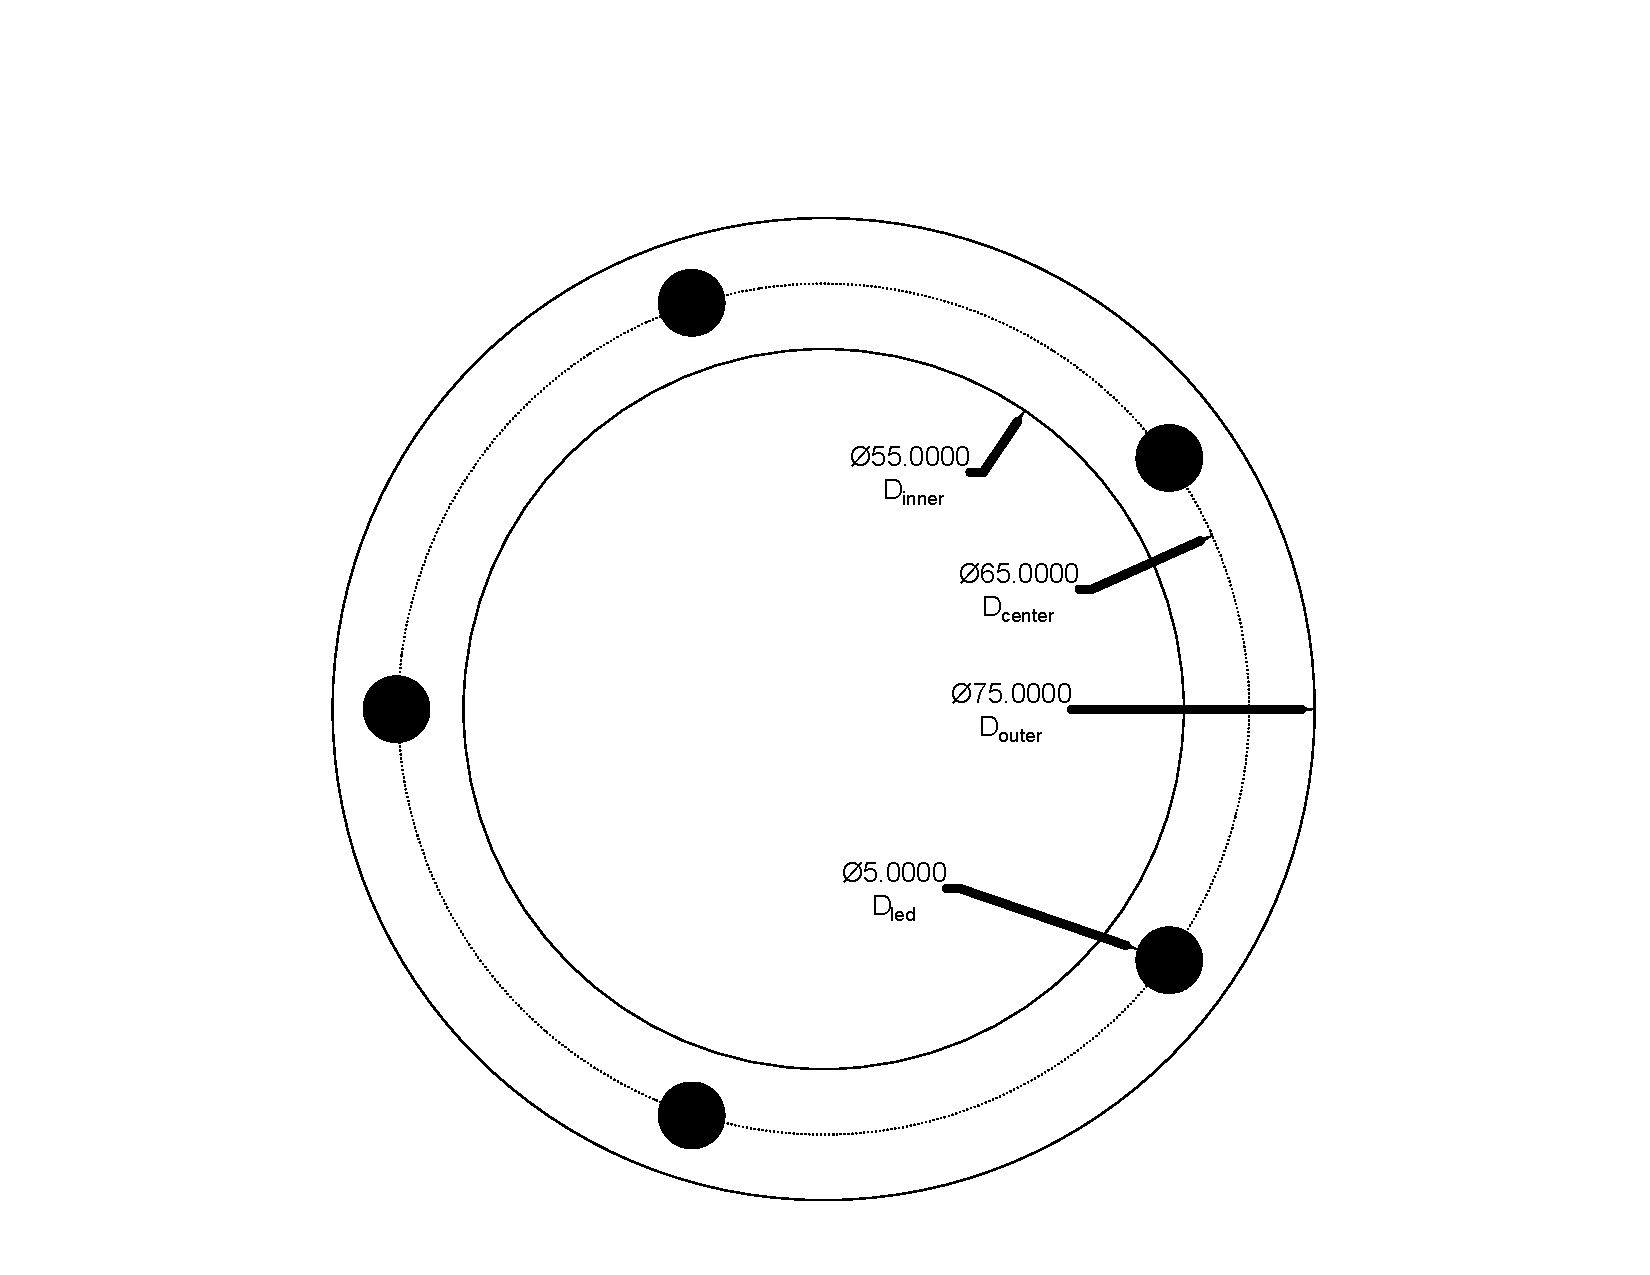
\includegraphics[width=0.6\textwidth,trim={2in 0.4in 2in 1.3in},clip, page=1]{Kravspecifikation/Ikke-funktionelle/graphics/LEDplacement.pdf}
    \caption{Skitse der viser de forskellige mål på en cup holder.}
    \label{fig:rap_LEDplacement}
\end{figure}
Af denne figur ses en skitse for, hvordan en CupHolder skal se ud, der er der, hvor en bruger skal placere en kop på. Her ses led'ernes placering, der stemmer overens med de specificerede mål på en kop, for at give den bedste lyseffekt i den gennemsigtige kop.\\\\
Herudover er der også lavet en skitse for den WebPage, hvor brugeren indtaster \textit{spiller oplysninger}. Denne kan ses af figur \ref{fig:rap_webpage_sketch}.

\begin{figure}[H]
    \centering
    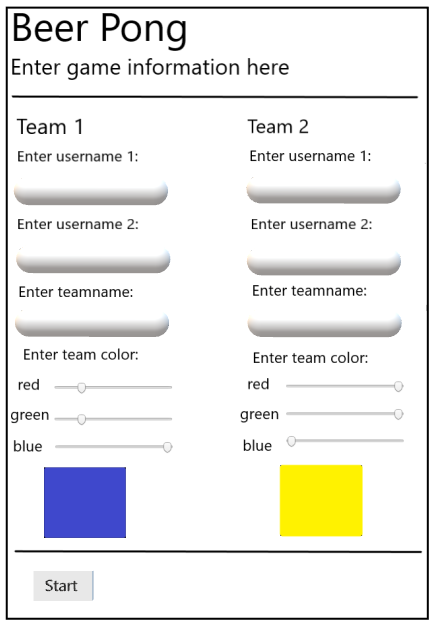
\includegraphics[width=0.6\textwidth]{Kravspecifikation/Ikke-funktionelle/graphics/WebPage_IF.png}
    \caption{Skitse af grænsefladen for WebPage}
   \label{fig:rap_webpage_sketch}
\end{figure}

Her ses den webpage, der anvendes i use casen \textit{UC1: Start Game}, hvor det kan ses, de forskellige felter til indtastning af spillerbrugernavne, holdnavne og trackbars til valg af holdfarve.

\end{document}